%\documentclass{standalone}
%\usepackage{tikz}
%\usetikzlibrary{patterns,plotmarks}
%\begin{document}
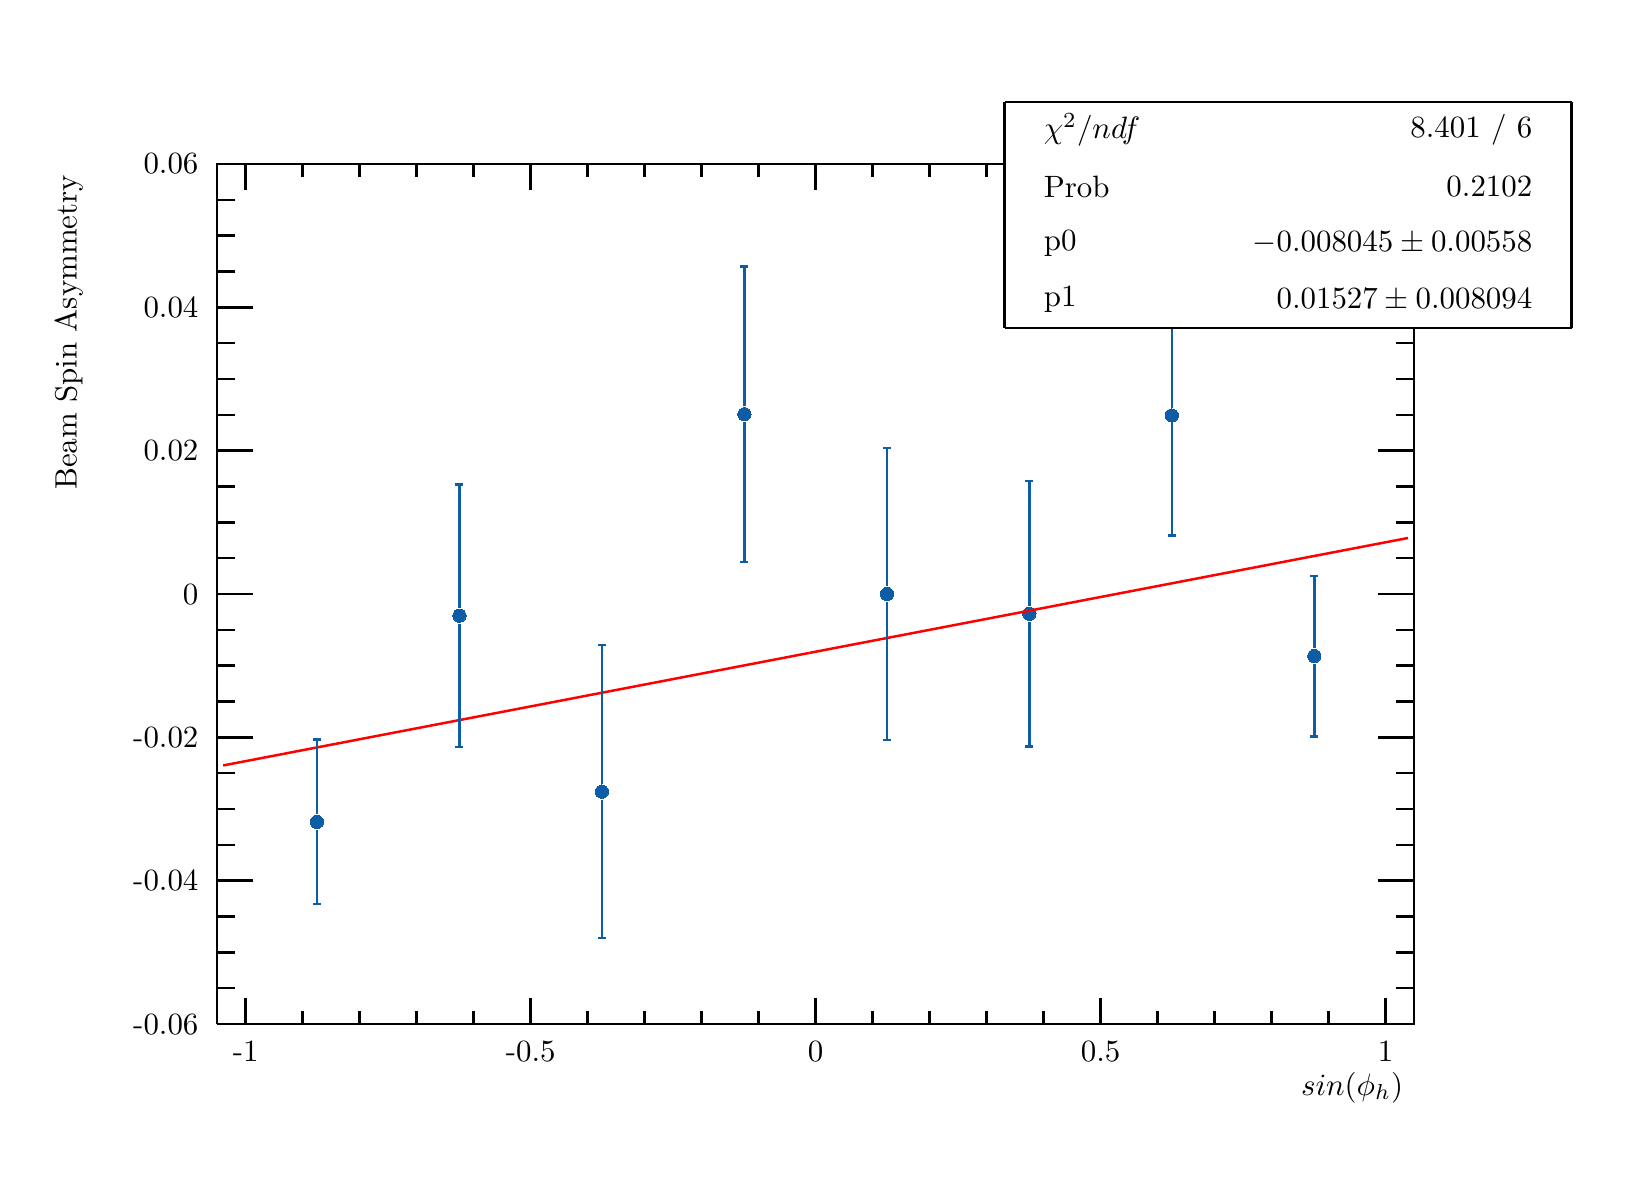
\begin{tikzpicture}
\def\CheckTikzLibraryLoaded#1{ \ifcsname tikz@library@#1@loaded\endcsname \else \PackageWarning{tikz}{usetikzlibrary{#1} is missing in the preamble.} \fi }
\CheckTikzLibraryLoaded{patterns}
\CheckTikzLibraryLoaded{plotmarks}
\pgfdeclareplotmark{cross} {
\pgfpathmoveto{\pgfpoint{-0.3\pgfplotmarksize}{\pgfplotmarksize}}
\pgfpathlineto{\pgfpoint{+0.3\pgfplotmarksize}{\pgfplotmarksize}}
\pgfpathlineto{\pgfpoint{+0.3\pgfplotmarksize}{0.3\pgfplotmarksize}}
\pgfpathlineto{\pgfpoint{+1\pgfplotmarksize}{0.3\pgfplotmarksize}}
\pgfpathlineto{\pgfpoint{+1\pgfplotmarksize}{-0.3\pgfplotmarksize}}
\pgfpathlineto{\pgfpoint{+0.3\pgfplotmarksize}{-0.3\pgfplotmarksize}}
\pgfpathlineto{\pgfpoint{+0.3\pgfplotmarksize}{-1.\pgfplotmarksize}}
\pgfpathlineto{\pgfpoint{-0.3\pgfplotmarksize}{-1.\pgfplotmarksize}}
\pgfpathlineto{\pgfpoint{-0.3\pgfplotmarksize}{-0.3\pgfplotmarksize}}
\pgfpathlineto{\pgfpoint{-1.\pgfplotmarksize}{-0.3\pgfplotmarksize}}
\pgfpathlineto{\pgfpoint{-1.\pgfplotmarksize}{0.3\pgfplotmarksize}}
\pgfpathlineto{\pgfpoint{-0.3\pgfplotmarksize}{0.3\pgfplotmarksize}}
\pgfpathclose
\pgfusepathqstroke
}
\pgfdeclareplotmark{cross*} {
\pgfpathmoveto{\pgfpoint{-0.3\pgfplotmarksize}{\pgfplotmarksize}}
\pgfpathlineto{\pgfpoint{+0.3\pgfplotmarksize}{\pgfplotmarksize}}
\pgfpathlineto{\pgfpoint{+0.3\pgfplotmarksize}{0.3\pgfplotmarksize}}
\pgfpathlineto{\pgfpoint{+1\pgfplotmarksize}{0.3\pgfplotmarksize}}
\pgfpathlineto{\pgfpoint{+1\pgfplotmarksize}{-0.3\pgfplotmarksize}}
\pgfpathlineto{\pgfpoint{+0.3\pgfplotmarksize}{-0.3\pgfplotmarksize}}
\pgfpathlineto{\pgfpoint{+0.3\pgfplotmarksize}{-1.\pgfplotmarksize}}
\pgfpathlineto{\pgfpoint{-0.3\pgfplotmarksize}{-1.\pgfplotmarksize}}
\pgfpathlineto{\pgfpoint{-0.3\pgfplotmarksize}{-0.3\pgfplotmarksize}}
\pgfpathlineto{\pgfpoint{-1.\pgfplotmarksize}{-0.3\pgfplotmarksize}}
\pgfpathlineto{\pgfpoint{-1.\pgfplotmarksize}{0.3\pgfplotmarksize}}
\pgfpathlineto{\pgfpoint{-0.3\pgfplotmarksize}{0.3\pgfplotmarksize}}
\pgfpathclose
\pgfusepathqfillstroke
}
\pgfdeclareplotmark{newstar} {
\pgfpathmoveto{\pgfqpoint{0pt}{\pgfplotmarksize}}
\pgfpathlineto{\pgfqpointpolar{44}{0.5\pgfplotmarksize}}
\pgfpathlineto{\pgfqpointpolar{18}{\pgfplotmarksize}}
\pgfpathlineto{\pgfqpointpolar{-20}{0.5\pgfplotmarksize}}
\pgfpathlineto{\pgfqpointpolar{-54}{\pgfplotmarksize}}
\pgfpathlineto{\pgfqpointpolar{-90}{0.5\pgfplotmarksize}}
\pgfpathlineto{\pgfqpointpolar{234}{\pgfplotmarksize}}
\pgfpathlineto{\pgfqpointpolar{198}{0.5\pgfplotmarksize}}
\pgfpathlineto{\pgfqpointpolar{162}{\pgfplotmarksize}}
\pgfpathlineto{\pgfqpointpolar{134}{0.5\pgfplotmarksize}}
\pgfpathclose
\pgfusepathqstroke
}
\pgfdeclareplotmark{newstar*} {
\pgfpathmoveto{\pgfqpoint{0pt}{\pgfplotmarksize}}
\pgfpathlineto{\pgfqpointpolar{44}{0.5\pgfplotmarksize}}
\pgfpathlineto{\pgfqpointpolar{18}{\pgfplotmarksize}}
\pgfpathlineto{\pgfqpointpolar{-20}{0.5\pgfplotmarksize}}
\pgfpathlineto{\pgfqpointpolar{-54}{\pgfplotmarksize}}
\pgfpathlineto{\pgfqpointpolar{-90}{0.5\pgfplotmarksize}}
\pgfpathlineto{\pgfqpointpolar{234}{\pgfplotmarksize}}
\pgfpathlineto{\pgfqpointpolar{198}{0.5\pgfplotmarksize}}
\pgfpathlineto{\pgfqpointpolar{162}{\pgfplotmarksize}}
\pgfpathlineto{\pgfqpointpolar{134}{0.5\pgfplotmarksize}}
\pgfpathclose
\pgfusepathqfillstroke
}
\definecolor{c}{rgb}{1,1,1};
\draw [color=c, fill=c] (0,0) rectangle (20,14.3719);
\draw [color=c, fill=c] (2.4,1.72462) rectangle (17.6,12.6472);
\definecolor{c}{rgb}{0,0,0};
\draw [c,line width=0.9] (2.4,1.72462) -- (2.4,12.6472) -- (17.6,12.6472) -- (17.6,1.72462) -- (2.4,1.72462);
\definecolor{c}{rgb}{1,1,1};
\draw [color=c, fill=c] (2.4,1.72462) rectangle (17.6,12.6472);
\definecolor{c}{rgb}{0,0,0};
\draw [c,line width=0.9] (2.4,1.72462) -- (2.4,12.6472) -- (17.6,12.6472) -- (17.6,1.72462) -- (2.4,1.72462);
\draw [c,line width=0.9] (2.4,1.72462) -- (17.6,1.72462);
\draw [c,line width=0.9] (2.7619,2.0523) -- (2.7619,1.72462);
\draw [c,line width=0.9] (3.48571,1.88846) -- (3.48571,1.72462);
\draw [c,line width=0.9] (4.20952,1.88846) -- (4.20952,1.72462);
\draw [c,line width=0.9] (4.93333,1.88846) -- (4.93333,1.72462);
\draw [c,line width=0.9] (5.65714,1.88846) -- (5.65714,1.72462);
\draw [c,line width=0.9] (6.38095,2.0523) -- (6.38095,1.72462);
\draw [c,line width=0.9] (7.10476,1.88846) -- (7.10476,1.72462);
\draw [c,line width=0.9] (7.82857,1.88846) -- (7.82857,1.72462);
\draw [c,line width=0.9] (8.55238,1.88846) -- (8.55238,1.72462);
\draw [c,line width=0.9] (9.27619,1.88846) -- (9.27619,1.72462);
\draw [c,line width=0.9] (10,2.0523) -- (10,1.72462);
\draw [c,line width=0.9] (10.7238,1.88846) -- (10.7238,1.72462);
\draw [c,line width=0.9] (11.4476,1.88846) -- (11.4476,1.72462);
\draw [c,line width=0.9] (12.1714,1.88846) -- (12.1714,1.72462);
\draw [c,line width=0.9] (12.8952,1.88846) -- (12.8952,1.72462);
\draw [c,line width=0.9] (13.619,2.0523) -- (13.619,1.72462);
\draw [c,line width=0.9] (14.3429,1.88846) -- (14.3429,1.72462);
\draw [c,line width=0.9] (15.0667,1.88846) -- (15.0667,1.72462);
\draw [c,line width=0.9] (15.7905,1.88846) -- (15.7905,1.72462);
\draw [c,line width=0.9] (16.5143,1.88846) -- (16.5143,1.72462);
\draw [c,line width=0.9] (17.2381,2.0523) -- (17.2381,1.72462);
\draw [c,line width=0.9] (2.7619,2.0523) -- (2.7619,1.72462);
\draw [c,line width=0.9] (17.2381,2.0523) -- (17.2381,1.72462);
\draw [anchor=base] (2.7619,1.25035) node[scale=1.11607, color=c, rotate=0]{-1};
\draw [anchor=base] (6.38095,1.25035) node[scale=1.11607, color=c, rotate=0]{-0.5};
\draw [anchor=base] (10,1.25035) node[scale=1.11607, color=c, rotate=0]{0};
\draw [anchor=base] (13.619,1.25035) node[scale=1.11607, color=c, rotate=0]{0.5};
\draw [anchor=base] (17.2381,1.25035) node[scale=1.11607, color=c, rotate=0]{1};
\draw [anchor= east] (17.6,0.919799) node[scale=1.11607, color=c, rotate=0]{$sin(\phi_{h})$};
\draw [c,line width=0.9] (2.4,12.6472) -- (17.6,12.6472);
\draw [c,line width=0.9] (2.7619,12.3196) -- (2.7619,12.6472);
\draw [c,line width=0.9] (3.48571,12.4834) -- (3.48571,12.6472);
\draw [c,line width=0.9] (4.20952,12.4834) -- (4.20952,12.6472);
\draw [c,line width=0.9] (4.93333,12.4834) -- (4.93333,12.6472);
\draw [c,line width=0.9] (5.65714,12.4834) -- (5.65714,12.6472);
\draw [c,line width=0.9] (6.38095,12.3196) -- (6.38095,12.6472);
\draw [c,line width=0.9] (7.10476,12.4834) -- (7.10476,12.6472);
\draw [c,line width=0.9] (7.82857,12.4834) -- (7.82857,12.6472);
\draw [c,line width=0.9] (8.55238,12.4834) -- (8.55238,12.6472);
\draw [c,line width=0.9] (9.27619,12.4834) -- (9.27619,12.6472);
\draw [c,line width=0.9] (10,12.3196) -- (10,12.6472);
\draw [c,line width=0.9] (10.7238,12.4834) -- (10.7238,12.6472);
\draw [c,line width=0.9] (11.4476,12.4834) -- (11.4476,12.6472);
\draw [c,line width=0.9] (12.1714,12.4834) -- (12.1714,12.6472);
\draw [c,line width=0.9] (12.8952,12.4834) -- (12.8952,12.6472);
\draw [c,line width=0.9] (13.619,12.3196) -- (13.619,12.6472);
\draw [c,line width=0.9] (14.3429,12.4834) -- (14.3429,12.6472);
\draw [c,line width=0.9] (15.0667,12.4834) -- (15.0667,12.6472);
\draw [c,line width=0.9] (15.7905,12.4834) -- (15.7905,12.6472);
\draw [c,line width=0.9] (16.5143,12.4834) -- (16.5143,12.6472);
\draw [c,line width=0.9] (17.2381,12.3196) -- (17.2381,12.6472);
\draw [c,line width=0.9] (2.7619,12.3196) -- (2.7619,12.6472);
\draw [c,line width=0.9] (17.2381,12.3196) -- (17.2381,12.6472);
\draw [c,line width=0.9] (2.4,1.72462) -- (2.4,12.6472);
\draw [c,line width=0.9] (2.856,1.72462) -- (2.4,1.72462);
\draw [c,line width=0.9] (2.628,2.17973) -- (2.4,2.17973);
\draw [c,line width=0.9] (2.628,2.63484) -- (2.4,2.63484);
\draw [c,line width=0.9] (2.628,3.08995) -- (2.4,3.08995);
\draw [c,line width=0.9] (2.856,3.54506) -- (2.4,3.54506);
\draw [c,line width=0.9] (2.628,4.00017) -- (2.4,4.00017);
\draw [c,line width=0.9] (2.628,4.45528) -- (2.4,4.45528);
\draw [c,line width=0.9] (2.628,4.91039) -- (2.4,4.91039);
\draw [c,line width=0.9] (2.856,5.36549) -- (2.4,5.36549);
\draw [c,line width=0.9] (2.628,5.8206) -- (2.4,5.8206);
\draw [c,line width=0.9] (2.628,6.27571) -- (2.4,6.27571);
\draw [c,line width=0.9] (2.628,6.73082) -- (2.4,6.73082);
\draw [c,line width=0.9] (2.856,7.18593) -- (2.4,7.18593);
\draw [c,line width=0.9] (2.628,7.64104) -- (2.4,7.64104);
\draw [c,line width=0.9] (2.628,8.09615) -- (2.4,8.09615);
\draw [c,line width=0.9] (2.628,8.55126) -- (2.4,8.55126);
\draw [c,line width=0.9] (2.856,9.00637) -- (2.4,9.00637);
\draw [c,line width=0.9] (2.628,9.46147) -- (2.4,9.46147);
\draw [c,line width=0.9] (2.628,9.91658) -- (2.4,9.91658);
\draw [c,line width=0.9] (2.628,10.3717) -- (2.4,10.3717);
\draw [c,line width=0.9] (2.856,10.8268) -- (2.4,10.8268);
\draw [c,line width=0.9] (2.628,11.2819) -- (2.4,11.2819);
\draw [c,line width=0.9] (2.628,11.737) -- (2.4,11.737);
\draw [c,line width=0.9] (2.628,12.1921) -- (2.4,12.1921);
\draw [c,line width=0.9] (2.856,12.6472) -- (2.4,12.6472);
\draw [anchor= east] (2.3,1.72462) node[scale=1.11607, color=c, rotate=0]{-0.06};
\draw [anchor= east] (2.3,3.54506) node[scale=1.11607, color=c, rotate=0]{-0.04};
\draw [anchor= east] (2.3,5.36549) node[scale=1.11607, color=c, rotate=0]{-0.02};
\draw [anchor= east] (2.3,7.18593) node[scale=1.11607, color=c, rotate=0]{0};
\draw [anchor= east] (2.3,9.00637) node[scale=1.11607, color=c, rotate=0]{0.02};
\draw [anchor= east] (2.3,10.8268) node[scale=1.11607, color=c, rotate=0]{0.04};
\draw [anchor= east] (2.3,12.6472) node[scale=1.11607, color=c, rotate=0]{0.06};
\draw [anchor= east] (0.519095,12.6472) node[scale=1.11607, color=c, rotate=90]{Beam Spin Asymmetry};
\draw [c,line width=0.9] (17.6,1.72462) -- (17.6,12.6472);
\draw [c,line width=0.9] (17.144,1.72462) -- (17.6,1.72462);
\draw [c,line width=0.9] (17.372,2.17973) -- (17.6,2.17973);
\draw [c,line width=0.9] (17.372,2.63484) -- (17.6,2.63484);
\draw [c,line width=0.9] (17.372,3.08995) -- (17.6,3.08995);
\draw [c,line width=0.9] (17.144,3.54506) -- (17.6,3.54506);
\draw [c,line width=0.9] (17.372,4.00017) -- (17.6,4.00017);
\draw [c,line width=0.9] (17.372,4.45528) -- (17.6,4.45528);
\draw [c,line width=0.9] (17.372,4.91039) -- (17.6,4.91039);
\draw [c,line width=0.9] (17.144,5.36549) -- (17.6,5.36549);
\draw [c,line width=0.9] (17.372,5.8206) -- (17.6,5.8206);
\draw [c,line width=0.9] (17.372,6.27571) -- (17.6,6.27571);
\draw [c,line width=0.9] (17.372,6.73082) -- (17.6,6.73082);
\draw [c,line width=0.9] (17.144,7.18593) -- (17.6,7.18593);
\draw [c,line width=0.9] (17.372,7.64104) -- (17.6,7.64104);
\draw [c,line width=0.9] (17.372,8.09615) -- (17.6,8.09615);
\draw [c,line width=0.9] (17.372,8.55126) -- (17.6,8.55126);
\draw [c,line width=0.9] (17.144,9.00637) -- (17.6,9.00637);
\draw [c,line width=0.9] (17.372,9.46147) -- (17.6,9.46147);
\draw [c,line width=0.9] (17.372,9.91658) -- (17.6,9.91658);
\draw [c,line width=0.9] (17.372,10.3717) -- (17.6,10.3717);
\draw [c,line width=0.9] (17.144,10.8268) -- (17.6,10.8268);
\draw [c,line width=0.9] (17.372,11.2819) -- (17.6,11.2819);
\draw [c,line width=0.9] (17.372,11.737) -- (17.6,11.737);
\draw [c,line width=0.9] (17.372,12.1921) -- (17.6,12.1921);
\draw [c,line width=0.9] (17.144,12.6472) -- (17.6,12.6472);
\definecolor{c}{rgb}{0.0470588,0.364706,0.647059};
\foreach \P in {(3.66667,4.29311), (5.47619,6.91149), (7.28571,4.67656), (9.09524,9.47019), (10.9048,7.18593), (12.7143,6.93621), (14.5238,9.45446), (16.3333,6.39801)}{\draw[mark options={color=c,fill=c},mark size=2.402402pt, line width=0.000000pt,
 mark=*] plot coordinates {\P};}
\definecolor{c}{rgb}{1,0,0};
\draw [c,line width=0.9] (2.476,5.00915) -- (2.628,5.03833) -- (2.78,5.06751) -- (2.932,5.09669) -- (3.084,5.12587) -- (3.236,5.15505) -- (3.388,5.18423) -- (3.54,5.21342) -- (3.692,5.2426) -- (3.844,5.27178) -- (3.996,5.30096) -- (4.148,5.33014) --
 (4.3,5.35932) -- (4.452,5.3885) -- (4.604,5.41768) -- (4.756,5.44686) -- (4.908,5.47605) -- (5.06,5.50523) -- (5.212,5.53441) -- (5.364,5.56359) -- (5.516,5.59277) -- (5.668,5.62195) -- (5.82,5.65113) -- (5.972,5.68031) -- (6.124,5.7095) --
 (6.276,5.73868) -- (6.428,5.76786) -- (6.58,5.79704) -- (6.732,5.82622) -- (6.884,5.8554) -- (7.036,5.88458) -- (7.188,5.91376) -- (7.34,5.94294) -- (7.492,5.97213) -- (7.644,6.00131) -- (7.796,6.03049) -- (7.948,6.05967) -- (8.1,6.08885) --
 (8.252,6.11803) -- (8.404,6.14721) -- (8.556,6.17639) -- (8.708,6.20557) -- (8.86,6.23476) -- (9.012,6.26394) -- (9.164,6.29312) -- (9.316,6.3223) -- (9.468,6.35148) -- (9.62,6.38066) -- (9.772,6.40984) -- (9.924,6.43902);
\draw [c,line width=0.9] (9.924,6.43902) -- (10.076,6.4682) -- (10.228,6.49739) -- (10.38,6.52657) -- (10.532,6.55575) -- (10.684,6.58493) -- (10.836,6.61411) -- (10.988,6.64329) -- (11.14,6.67247) -- (11.292,6.70165) -- (11.444,6.73084) --
 (11.596,6.76002) -- (11.748,6.7892) -- (11.9,6.81838) -- (12.052,6.84756) -- (12.204,6.87674) -- (12.356,6.90592) -- (12.508,6.9351) -- (12.66,6.96428) -- (12.812,6.99347) -- (12.964,7.02265) -- (13.116,7.05183) -- (13.268,7.08101) --
 (13.42,7.11019) -- (13.572,7.13937) -- (13.724,7.16855) -- (13.876,7.19773) -- (14.028,7.22691) -- (14.18,7.2561) -- (14.332,7.28528) -- (14.484,7.31446) -- (14.636,7.34364) -- (14.788,7.37282) -- (14.94,7.402) -- (15.092,7.43118) --
 (15.244,7.46036) -- (15.396,7.48955) -- (15.548,7.51873) -- (15.7,7.54791) -- (15.852,7.57709) -- (16.004,7.60627) -- (16.156,7.63545) -- (16.308,7.66463) -- (16.46,7.69381) -- (16.612,7.72299) -- (16.764,7.75218) -- (16.916,7.78136) --
 (17.068,7.81054) -- (17.22,7.83972) -- (17.372,7.8689);
\draw [c,line width=0.9] (17.372,7.8689) -- (17.524,7.89808);
\definecolor{c}{rgb}{1,1,1};
\draw [color=c, fill=c] (12.4,10.5633) rectangle (19.6,13.4377);
\definecolor{c}{rgb}{0,0,0};
\draw [c,line width=0.9] (12.4,10.5633) -- (19.6,10.5633);
\draw [c,line width=0.9] (19.6,10.5633) -- (19.6,13.4377);
\draw [c,line width=0.9] (19.6,13.4377) -- (12.4,13.4377);
\draw [c,line width=0.9] (12.4,13.4377) -- (12.4,10.5633);
\draw [anchor= west] (12.76,13.0784) node[scale=1.11607, color=c, rotate=0]{$\chi^{2} / ndf $};
\draw [anchor= east] (19.24,13.0784) node[scale=1.11607, color=c, rotate=0]{ 8.401 / 6};
\draw [anchor= west] (12.76,12.3598) node[scale=1.11607, color=c, rotate=0]{Prob  };
\draw [anchor= east] (19.24,12.3598) node[scale=1.11607, color=c, rotate=0]{ 0.2102};
\draw [anchor= west] (12.76,11.6412) node[scale=1.11607, color=c, rotate=0]{p0       };
\draw [anchor= east] (19.24,11.6412) node[scale=1.11607, color=c, rotate=0]{$ -0.008045 \pm 0.00558$};
\draw [anchor= west] (12.76,10.9226) node[scale=1.11607, color=c, rotate=0]{p1       };
\draw [anchor= east] (19.24,10.9226) node[scale=1.11607, color=c, rotate=0]{$ 0.01527 \pm 0.008094$};
\definecolor{c}{rgb}{0.0470588,0.364706,0.647059};
\draw [c,line width=0.9] (3.66667,4.39361) -- (3.66667,5.33837);
\draw [c,line width=0.9] (3.66667,4.19261) -- (3.66667,3.24785);
\draw [c,line width=0.9] (3.61642,5.33837) -- (3.71692,5.33837);
\draw [c,line width=0.9] (3.61642,3.24785) -- (3.71692,3.24785);
\draw [c,line width=0.9] (5.47619,7.01199) -- (5.47619,8.57749);
\draw [c,line width=0.9] (5.47619,6.81099) -- (5.47619,5.2455);
\draw [c,line width=0.9] (5.42594,8.57749) -- (5.52644,8.57749);
\draw [c,line width=0.9] (5.42594,5.2455) -- (5.52644,5.2455);
\draw [c,line width=0.9] (7.28571,4.77706) -- (7.28571,6.53686);
\draw [c,line width=0.9] (7.28571,4.57606) -- (7.28571,2.81626);
\draw [c,line width=0.9] (7.23546,6.53686) -- (7.33597,6.53686);
\draw [c,line width=0.9] (7.23546,2.81626) -- (7.33597,2.81626);
\draw [c,line width=0.9] (9.09524,9.57069) -- (9.09524,11.3474);
\draw [c,line width=0.9] (9.09524,9.36968) -- (9.09524,7.59295);
\draw [c,line width=0.9] (9.04499,11.3474) -- (9.14549,11.3474);
\draw [c,line width=0.9] (9.04499,7.59295) -- (9.14549,7.59295);
\draw [c,line width=0.9] (10.9048,7.28643) -- (10.9048,9.04236);
\draw [c,line width=0.9] (10.9048,7.08543) -- (10.9048,5.3295);
\draw [c,line width=0.9] (10.8545,9.04236) -- (10.955,9.04236);
\draw [c,line width=0.9] (10.8545,5.3295) -- (10.955,5.3295);
\draw [c,line width=0.9] (12.7143,7.03672) -- (12.7143,8.6218);
\draw [c,line width=0.9] (12.7143,6.83571) -- (12.7143,5.25062);
\draw [c,line width=0.9] (12.664,8.6218) -- (12.7645,8.6218);
\draw [c,line width=0.9] (12.664,5.25062) -- (12.7645,5.25062);
\draw [c,line width=0.9] (14.5238,9.55497) -- (14.5238,10.9776);
\draw [c,line width=0.9] (14.5238,9.35396) -- (14.5238,7.93129);
\draw [c,line width=0.9] (14.4736,10.9776) -- (14.5741,10.9776);
\draw [c,line width=0.9] (14.4736,7.93129) -- (14.5741,7.93129);
\draw [c,line width=0.9] (16.3333,6.49851) -- (16.3333,7.41751);
\draw [c,line width=0.9] (16.3333,6.29751) -- (16.3333,5.37851);
\draw [c,line width=0.9] (16.2831,7.41751) -- (16.3836,7.41751);
\draw [c,line width=0.9] (16.2831,5.37851) -- (16.3836,5.37851);
\definecolor{c}{rgb}{1,1,1};
\draw [color=c, fill=c] (12.4,10.5633) rectangle (19.6,13.4377);
\definecolor{c}{rgb}{0,0,0};
\draw [c,line width=0.9] (12.4,10.5633) -- (19.6,10.5633);
\draw [c,line width=0.9] (19.6,10.5633) -- (19.6,13.4377);
\draw [c,line width=0.9] (19.6,13.4377) -- (12.4,13.4377);
\draw [c,line width=0.9] (12.4,13.4377) -- (12.4,10.5633);
\draw [anchor= west] (12.76,13.0784) node[scale=1.11607, color=c, rotate=0]{$\chi^{2} / ndf $};
\draw [anchor= east] (19.24,13.0784) node[scale=1.11607, color=c, rotate=0]{ 8.401 / 6};
\draw [anchor= west] (12.76,12.3598) node[scale=1.11607, color=c, rotate=0]{Prob  };
\draw [anchor= east] (19.24,12.3598) node[scale=1.11607, color=c, rotate=0]{ 0.2102};
\draw [anchor= west] (12.76,11.6412) node[scale=1.11607, color=c, rotate=0]{p0       };
\draw [anchor= east] (19.24,11.6412) node[scale=1.11607, color=c, rotate=0]{$ -0.008045 \pm 0.00558$};
\draw [anchor= west] (12.76,10.9226) node[scale=1.11607, color=c, rotate=0]{p1       };
\draw [anchor= east] (19.24,10.9226) node[scale=1.11607, color=c, rotate=0]{$ 0.01527 \pm 0.008094$};
\end{tikzpicture}
%\end{document}
